\chapter{Architecture Description}

% This doesnt have to be a section
\section{Overall description}

The MANGO project aims at allowing developers to easily develop applications that target different types of accelerator architectures. In particular,  three types of accelerators are considered: symmetric multiprocessors, which are characterized by good capabilities in terms of OS support and execution flexibility (i.e., they are able to run a POSIX-compliant runtime); GPGPU-like accelerators, which are programmable but are not able to run a fully compliant POSIX runtime; and hardware accelerators, which do not need or support any kind  of software runtime. Applications, on the other hand, may be developed either by domain experts with limited knowledge of parallel computing and programming models, or by more experienced programmers. 

Thus, the following requirements arise:
\begin{itemize}
    \item 
    Supporting the use of industry-standard programming models for heterogeneous systems, such as OpenCL, while guaranteeing functional portability across different programmable accelerators, as well as host-side compatibility for all accelerators and automated resource management;
    \item 
    Supporting a simple fork-join model, on which application developers not willing to use OpenCL can map their applications;
    \item
    Supporting future extensions of the MANGO software stack to support skeleton-based programming.
\end{itemize}

The user-facing module (Libmango), therefore, needs to operate in a way that is akin to an intermediate language in a compiler: it must allow the software stack developers to easily map high-level programming models on the range of supported accelerators, while providing at least functional compatibility. Depending on the individual capabilities of each accelerator, the low-level runtime system should also introduce optimizations or additional features; this would indeed cause compatibility issues, but it would also allow developers to implement specialized versions of their applications for any given accelerator. \cite{mango_exploring_manycore_architectures}

%TODO better diagram
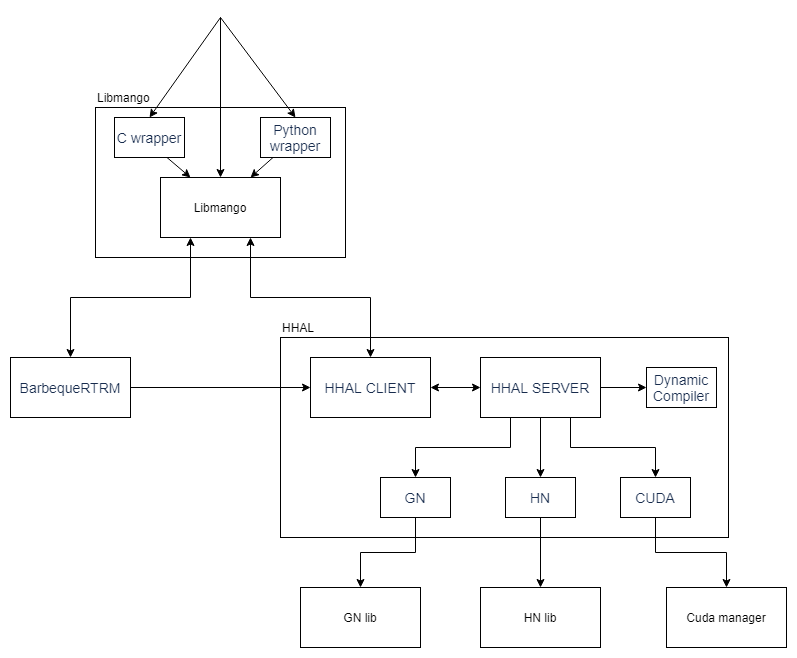
\includegraphics[scale=0.5]{img/architecture.png}

\section{Core elements}
Throughout the multiple MANGO modules, there are a few core elements often present. These are the components necessary to specify and control an user application and its execution. Although their names may vary from module to module, here they are defined as Kernel, Memory Buffer, Event and Task graph.

\subsubsection{Kernel}
In computing, a compute kernel is a routine compiled for high throughput accelerators (such as graphics processing units (GPUs), digital signal processors (DSPs) or field-programmable gate arrays (FPGAs)), separate from but used by a main program (typically running on a central processing unit). \cite{kernel_wikipedia}

The MANGO system manages user defined Kernels and their execution. For a particular Kernel, multiple sources (accelerator specific implementations of the kernel) can be specified. The architectures for which an implementation is available are considered in the kernel-accelerator assignation process by the resource manager. 

As any computer program, a kernel must have the capability of interacting with the outside world in order to perform significant work. This is achieved through the support of kernel arguments.

%TODO styling
Three types of kernel arguments are supported: 
\begin{itemize}
    \item Scalar Argument: A scalar value. For example, an integer.
    \item Buffer Argument: A pointer to a Memory Buffer.
    \item Event Argument: A pointer to an Event data type.
\end{itemize}

\subsubsection{Memory Buffer}
%TODO better diagram
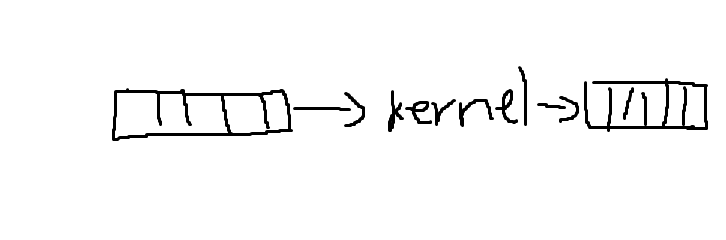
\includegraphics[scale=0.5]{img/kernel_buffer.png}

In computer science, a data buffer (or just buffer) is a region of a physical memory storage used to temporarily store data while it is being moved from one place to another. \cite{buffer_wikipedia}

Kernels read from Input Buffers and write to Output Buffers for inter-kernel and host-kernel data transfering.

A Memory Buffer is defined by the user and allocated by MANGO at the target architectures, where a Kernel that makes use of said Buffer (as either input or output) is assigned.

\subsubsection{Event}

An event is a data structure utilized for communication and synchronization of different parts of the system.

User defined events can be accessed by Kernels through Event Arguments, providing the user with the necessary tools for the implementation of host-kernel or inter-kernel synchronization.

By default, MANGO utilizes kernel termination events for both internal and host synchronization.

\subsubsection{Task Graph}

The Task Graph gives a global picture of the application's behaviour and represents data and control dependencies between Kernels, Memory Buffers and Events. The Task Graph provides the resource manager with the information needed to generate the best feasible resource allocation for the requested QoS. \cite{mango_exploring_manycore_architectures}


\section{Libmango}
Libmango is the front-facing module of the MANGO system, hence providing the system's API for user interaction with the underlying components, and acting as an abstraction layer between user defined models and module specific requirements.

The goal of the Libmango module is to allow software stack developers to easily map high-level programming models on the range of supported accelerators. Through the communication with the BarbecueRTRM and HHAL modules, user models are automatically mapped to the supported accelerators in a transparent manner, removing integration complexity from the user's hands.

The Libmango API allows developers to indicate to the runtime the components of their application, namely kernels, memory buffers and events. These are grouped in a task-graph that represents the dependencies among the multiple components. 

\subsection{Context}
The Context is the main class in the Libmango module, it holds the state information of the host side runtime for a single application, and its created by the user at the beginning of their interaction with an application name and a recipe file needed by BarbecueRTRM for the resource allocation. Every subsequent component (kernels, buffers, events and task graph) has to be registered in the Context in order to be considered part of the application.

Once the application is specified, the task graph information is sent to the BarbecueRTRM for the resource allocation. After a successful resource allocation, the application is now ready to run.

\subsection{Kernel management}
Libmango exposes functionalities and data structures that can be used to represent and manipulate kernels.

Kernels are identified by an user-provided integer. For a single kernel, multiple implementations can be specified, each one targeting a different supported accelerator and thus provided in their respective architecture's requirements - a kernel implementation targeting an NVIDIA GPGPU would require a CUDA implementation.
Kernel versions (implementations) are stored either in memory or in external files. According to the targeted architecture, multiple source types are supported. The kernel source can be a pre-compiled binary file or code in accelerator-supported language, provided via a string stored in memory or a source file, to be dynamically compiled if required.
The resource manager will rely on the available options in the assignation of kernels to accelerators.

Kernels can be manually started by the developer once the resource allocation is successfully completed.

Libmango supports three types of kernel arguments: Scalar arguments, Buffer arguments and Event arguments.
These essentially act as wrappers of the HHAL kernel arguments.

\subsubsection{Scalar argument}
A Scalar argument consists of a scalar value. The types supported by Libmango are signed and unsigned integers of sizes 8, 16, 32 and 64; as well as float values.
When a Scalar argument is created, the provided value is copied and stored in memory, and later sent to the HHAL module when their respective kernel is run. 

\subsubsection{Buffer argument}
A Buffer argument consists of a Buffer integer identifier. The corresponding memory pointer in the accelerator's memory space is passed as an argument to the Kernel at execution time.

%TODO better explain how the kernel function receives the event argument depending on the architecture
\subsubsection{Event argument}
An Event argument consists of an Event integer identifier. The corresponding Event is passed as an argument to the Kernel at execution time.


\subsection{Buffer management}
Libmango exposes functionalities and data structures that can be used to represent and manipulate Memory Buffers.

A Buffer is identified by an user-provided integer, and consists of a pointer to a memory location where the Memory Buffer starts, and its size in bytes. 
To define a Buffer, the user needs to register it to the application's Context. A Buffer is allocated in the same accelerator where the Kernel that writes to, or reads from it, is assigned by the resource manager.
Once successfully allocated, Libmango permits the writing of the Buffer with host-side data, as well as reading from the Buffer into host memory.


\subsection{Event management}


\section{BarbecueRTRM}

\section{HHAL}

\section{CUDA Manager}

\section{HN}

\section{GN}